\documentclass[letterpaper,11pt]{article}
\oddsidemargin -1.0cm \textwidth 17.5cm

\usepackage[utf8]{inputenc}
\usepackage[activeacute,spanish, es-lcroman]{babel}
\decimalpoint
\usepackage{amsfonts,setspace}
\usepackage{amsmath}
\usepackage{amssymb, amsmath, amsthm}
\usepackage{comment}
\usepackage{float}
\usepackage{amssymb}
\usepackage{dsfont}
\usepackage{anysize}
\usepackage{multicol}
\usepackage{enumerate}
\usepackage{graphicx}
\usepackage[left=1.5cm,top=2cm,right=1.5cm, bottom=1.7cm]{geometry}
\setlength\headheight{1.5em} 
\usepackage{fancyhdr}
\usepackage{multicol}
\usepackage{hyperref}
\usepackage{wrapfig}
\usepackage{subcaption}
\usepackage{siunitx}
\usepackage{cancel}
\usepackage{mdwlist}
\usepackage{svg}
\pagestyle{fancy}
\fancyhf{}
\renewcommand{\labelenumi}{\normalsize\bfseries P\arabic{enumi}.}
\renewcommand{\labelenumii}{\normalsize\bfseries (\alph{enumii})}
\renewcommand{\labelenumiii}{\normalsize\bfseries \roman{enumiii})}


\begin{document}

\fancyhead[L]{\itshape{Facultad de Ciencias F\'isicas y Matem\'aticas}}
\fancyhead[R]{\itshape{Universidad de Chile}}
\rfoot[]{pág. \thepage}

\begin{minipage}{11.5cm}
    \begin{flushleft}
        \hspace*{-0.6cm}\textbf{FI1000 Introducción a la Física Clásica}\\
        \hspace*{-0.6cm}\textbf{Tutor:} Alejandro Cartes
    \end{flushleft}
\end{minipage}

\begin{picture}(2,3)
    \put(366, -10){
\includegraphics[scale=0.9]{2020-1/Imágenes/logo/dfi-fcfm.pdf}}
\end{picture}

\begin{center}
	\LARGE\textbf{Tutoría Examen}
\end{center}

\vspace{-1cm}
\begin{enumerate}\setlength{\itemsep}{0.4cm}

\item[]

\item \textbf{[Estática]} Una barra homogénea de largo $L$ y masa $M$ reposa con un extremo fijo en un pivote en el suelo y el otro sostenido por una cuerda ideal, en donde los ángulos formados ($\alpha$, $\beta$) son conocidos.
    \begin{enumerate}
        \item Determine la tensión de la cuerda
        
        \item Determine el tamaño de la reacción en el punto de apoyo
    \end{enumerate}

    \begin{figure}[h!]
      \centering
      \svgpath{../../2021-1/Imagenes/aux13}
      \includesvg[width=0.35\linewidth]{barra.svg}
    \end{figure}

\item \textbf{[Estática + Hidrostática]} Considere una varilla homogénea de largo $L$, sección transversal $A$ y densidad de masa $\rho$, tocando el fondo de un recipiente que contiene dos líquidos de densidades $\rho_1$ y $\rho_2$, con $\rho_1 < \rho_2$. Las alturas de cada líquido en el recipiente son $h_1$ y $h_2$, respectivamente.
Encuentre el ángulo $\theta$ con la horizontal que forma la varilla cuando está en equilibrio

\begin{figure}[H]
    \centering
    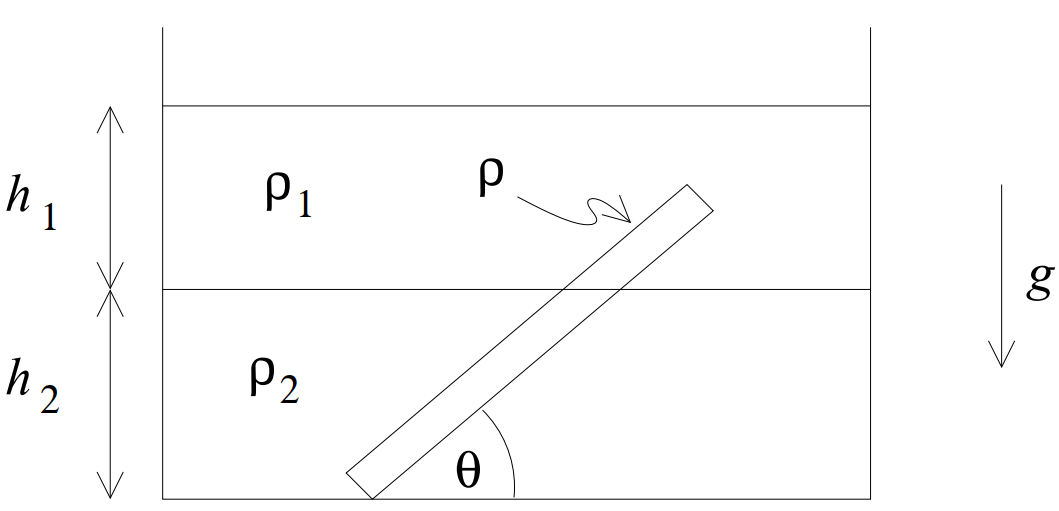
\includegraphics[width=0.5\linewidth]{tutorías/2023/img/empuje.png}
\end{figure}

\item \textbf{[Mov. Circular + Energía]}  Un esquiador de masa $m$ realiza un salto durante los Juegos Olímpicos de Invierno en la siguiente pista partiendo del reposo:
\begin{multicols}{2}
Despreciando cualquier roce entre las superficies y con el aire:

\begin{enumerate}
    \item Encuentre la aceleración total del esquiador en el punto de despegue de la pista

    \item Determine la máxima altura que alcanza luego de saltar
\end{enumerate}

\columnbreak

\begin{figure}[H]
    \centering
    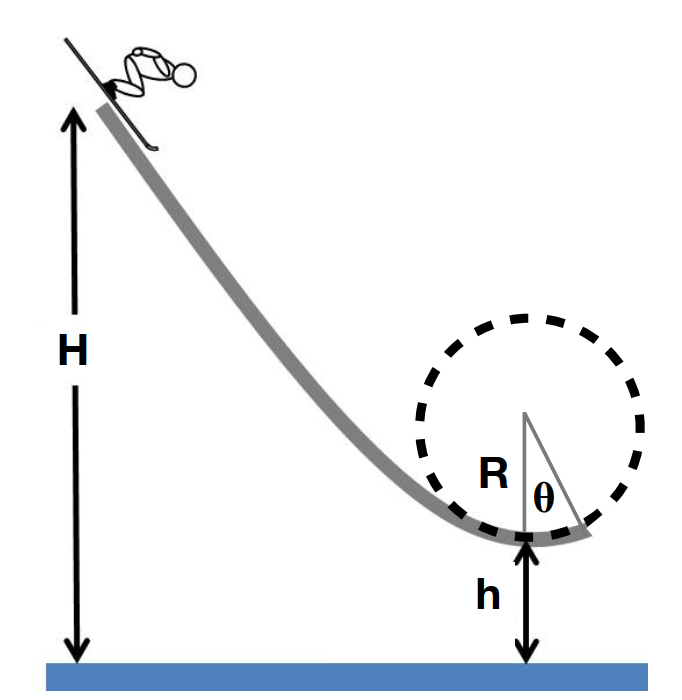
\includegraphics[width=0.4\linewidth]{tutorías/2023/img/ski.png}
\end{figure}

\end{multicols}
\item \textbf{[Dinámica + Cinemática]} Un objeto de masa $m_1$ se deja caer desde el punto más alto de un plano inclinado, el cual forma un ángulo $\theta$ con la horizontal y tiene altura máxima $h$. El plano inclinado está a su vez sobre un bloque rectangular de altura $H$ con respecto al suelo. El plano inclinado y el bloque se encuentran firmemente adosados entre sí y al suelo, de manera que no se mueven debido al movimiento de $m_1$. Si los coeficientes de roce estático y cinético entre $m_1$ y el plano inclinado son $\mu_e$ y $\mu_d$, respectivamente. 

\begin{enumerate}
    \item Determine la magnitud de la aceleración de $m_1$ a lo largo de su movimiento sobre el plano inclinado

    \item Determine la rapidez con que $m_1$ sale del plano

    \item Determine la distancia $R$ a la que $m_1$ golpea el suelo, con respecto a la base del bloque
\end{enumerate}

\begin{figure}[H]
    \centering
    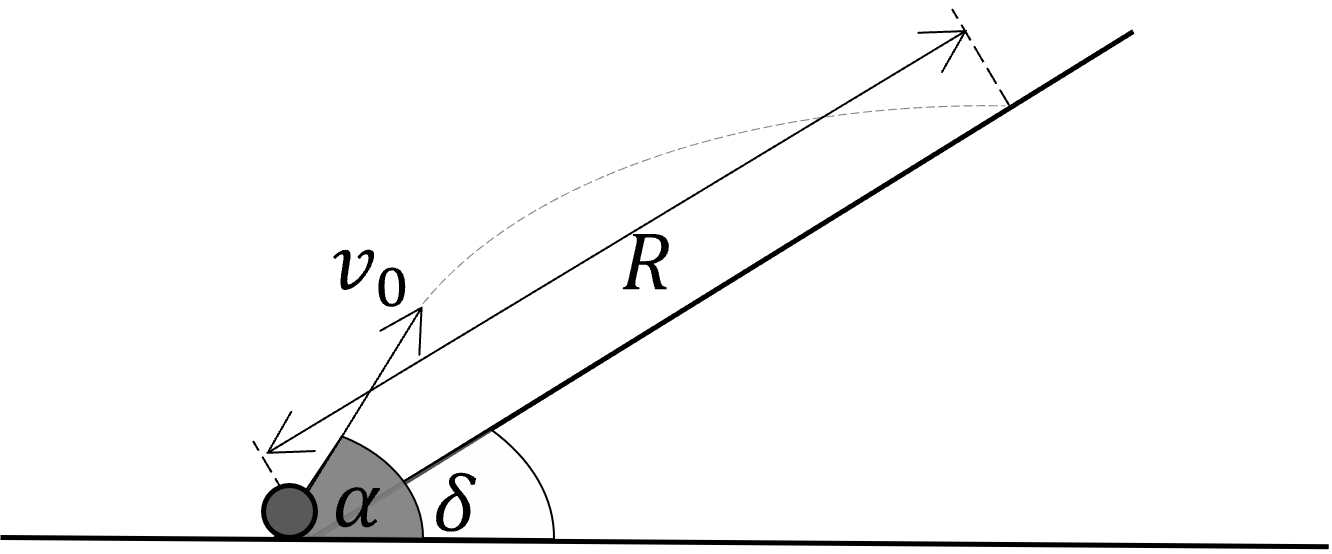
\includegraphics[width=0.6\linewidth]{tutorías/2023/img/plano.png}
\end{figure}

% Para imágenes vectoriales -> el texto tiene que estar en LaTeX
% \begin{figure}[htbp]
%   \centering
%   \svgpath{../Imagenes/ejercicios}  -> .. irse pa'trás 
%   \includesvg{ej5.svg}
% \end{figure}

\end{enumerate}
\end{document}
